\section{Infrastructure and Workflow}\label{sec:infrastructure}

Having established the tool requirements, we now detail the implementation of our workflow along with the minimal infrastructure necessary to sustain it.

In figure~\ref{fig:project-infra}, we describe our infrastructure that can be first deployed on a local Kubernetes single node cluster
with independent DataOps and MLOps pipelines develop by potentially different teams with different roles.

\begin{figure}[!htbp]
    \centering
    \caption{Proposed MLOps Kubernetes infrastructure using GitOps principles}
    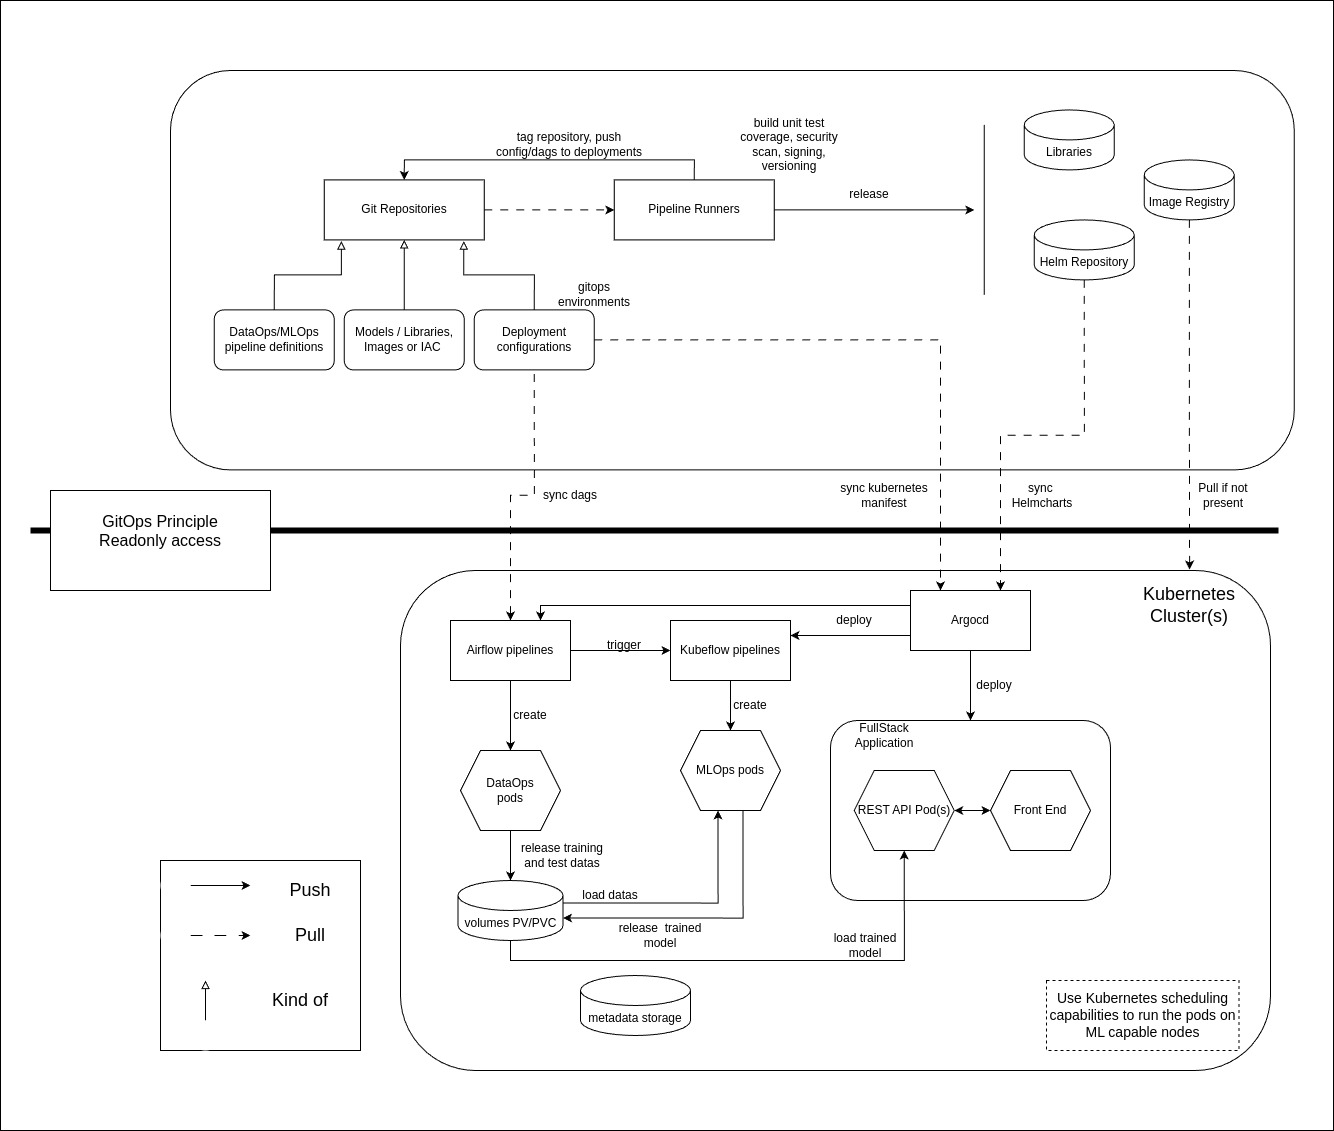
\includegraphics[scale=0.35]{images/project/mthmlops-infra}
    \label{fig:project-infra}
\end{figure}

By using Airflow pipelines as general pipelines to trigger our Kubeflow pipelines, we can easily gain in maturity towards
more automation by combining the DataOps pipelines and MLOps pipelines together when they are mature enough.

This way we enable kubeflow features for our model developers within a more general purpose environment.

By using the git-sync capabilities of Airflow we can synchronise our dags directly with airflow and
even trigger them automatically in a later stage towards automation.

Notably our infrastructure shows the GitOps pull based strategy.
Only the GitHub actions runners do pushes to other git repositories or other
storage like HelmChart repository, images repository or any library repository.
Our Kubernetes environments only pull changes from those repositories, making our infrastructure fully private and easily deployable anywhere.
We will now further describe the component of our workflow.

\subsection{General workflow}\label{subsec:general-development-workflow}
As previously outlined in our state-of-the-art review, the primary triggers for initiating our workflow are either
the emergence of a new development need or the availability of new data.
Beyond the initial phase—during which the project is discussed and defined in collaboration with business stakeholders.
The motivation for further development or model retraining typically arises from the system's monitoring and feedback loops.

Within our GitOps-based MLOps workflow, any change whether in code or configuration must be committed to the appropriate Git repository.
Each push to the repository triggers a DevOps pipeline, responsible for building images, running unit tests and releasing images.
This part culminate in updating configuration files in a dedicated configuration repository.
This repository is continuously monitored and synchronised by ArgoCD or Airflow, which applies the changes to the cluster and initiates the DataOps pipeline
or integration tests.
Upon successful completion of this stage, the MLOps pipeline is triggered.
If the newly trained model passes validation criteria, it is released to a model repository.
In accordance with GitOps principles, the deployment involves updating configuration files in a separate Git repository,
enabling ArgoCD to automatically deploy the new model version to the production environment thus closing the automation loop
as shown in figure~\ref{fig:general-workflow}.
By applying a GitOps strategy to both our development projects and infrastructure as code,
we establish a fully GitOps-driven infrastructure that can consistently deploy our applications and infrastructure across any environment.

\begin{figure}[!htbp]
    \centering
    \caption{General Workflow}
    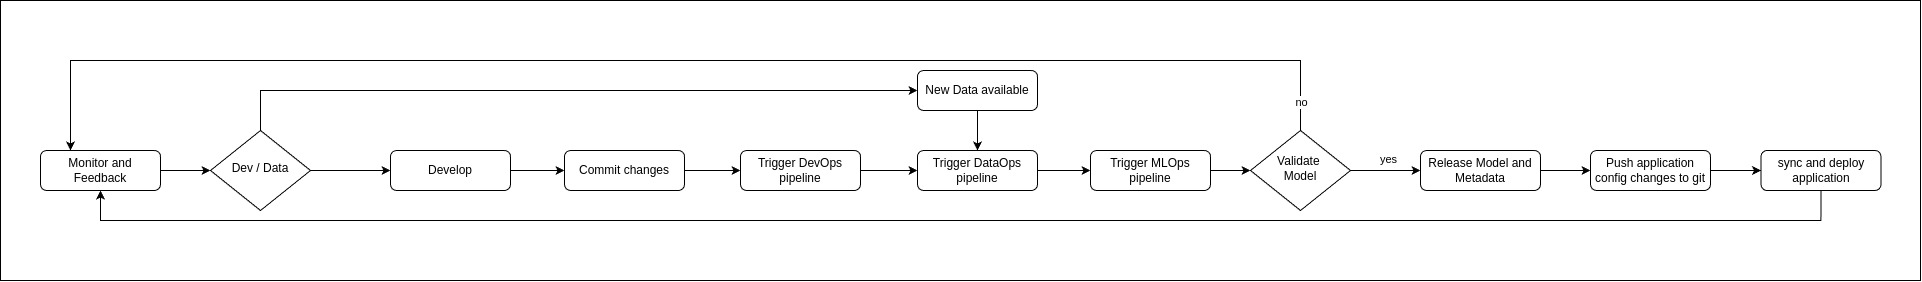
\includegraphics[width=\linewidth]{images/project/general_workflow}
    \label{fig:general-workflow}
\end{figure}

\subsection{Git Repositories}\label{subsec:git-repositories}
As mentioned, we use Git repositories for version control and to trigger our DevOps pipelines.
Additionally, they serve as a way to distribute responsibilities and coordinate work across teams within our MLOps project.
Using GitHub’s access management features, we are able to effectively manage these workflows and permissions.

Within our infrastructure, we consider 4 types of Git Repositories: Code, MLOps/DataOps pipelines, Deployment/Configuration, DevOps pipelines templates.

Following GitOps principle those are the source of truth for all our code and configurations, for the infrastructure, the pipelines, the model and the software development.


\subsubsection{Code Repositories}
that holds code for models, libraries, docker images and infrastructure as code using Helm.

\subsubsection{MLOps and DataOps Pipelines Repositories}
In our infrastructure those repositories holds the definition of our Airflow DAGs.
In the first iteration those repositories can also hold images for.

We adopt a consistent structure (figure~\ref{fig:sidebyside}) for both our DataOps and MLOps pipeline repositories, incorporating a config.yml file that mirrors the organizational pattern of Helm chart project (values.yaml).
In both cases, an images directory is used to define containerized steps for the pipelines and for deployment configurations within the Helm charts.
This consistency permit to reuse our Devops pipelines templates.

\begin{figure}[h!]
    \centering
    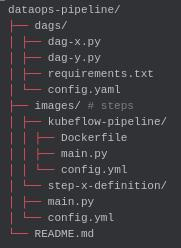
\includegraphics[scale=0.35]{images/project/git-repo-dataops}
    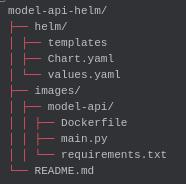
\includegraphics[scale=0.35]{images/project/git-repo-helm}
    \caption{Consistent structure within repositories}
    \label{fig:sidebyside}
\end{figure}


\subsubsection{Deployment/Configuration repositories}
Those repositories are used to hold configuration for the deployed applications and Airflow dags.
We use ArgoCD GitOps implementation to synchronise changes to those repositories.
Airflow git/sync feature allows us to synchronise our dags with
Change in those repositories can be automated by the pipeline runners.
Depending on your team and organization those repositories can be separated into multiple repositories (per team, per domain, per environment (dev,test,staging,prod))
For the Dev environment we allow developers to push from their code repositories within those repositories.
For the production environment we use a pipeline to pull the configuration from the staging environment.
Production environments can be manage by an Operation team to approve and manage those deployment
according to organization policies.
We called this promote our configuration to a new environment.
In case of full automation the pulling/promotion can be trigger automatically by ArgoCD sending webhooks on any test results desired.

\subsubsection{CI/CD pipelines templates}
In those we define DevOps workflows that can be used in any repository to be used by the developers.
It includes building image workflows, versioning with tags on repositories, pushing new configurations into deployments repositories.
By defining them in a separate repository it allows us to version them and make it easy for developers to choose a workflow.
Each workflow is closely tight to the structure of the repository, so we defined one per type of repositories.


\subsubsection{General Rules for Managing our Git Repositories}
We follow the GitHub flow with adaptations to fit our workflow.
However, these rules can be adjusted as needed, and our project is not strictly bound to them.
They are necessary, though, to enable automation alongside human review through approval gates.

\begin{itemize}
    \item A Pull Request is required for merging into the \texttt{main} branch, including a pipeline run and team review.
    \item Follow GitHub flow, using \texttt{feature/} and \texttt{hotfix/} branches for development.
    \item Approvals are required for deploying to environment-specific repositories.
    \item The \texttt{main} branch is deployed to the production environment or released into production Docker/Helm repositories.
    \item Other branches are deployed sequentially to all environments, passing tests and approval gates before merging to main.
\end{itemize}

\subsection{GitOps}\label{subsec:gitops2}
With a Helm-based installation pipeline, the runner requires write access to push applications directly to Kubernetes.
By adopting ArgoCD and a GitOps approach, we eliminate this requirement by pulling changes directly from GitHub.
This enables all operations to be managed within GitHub.
However, it necessitates properly configured permissions in GitHub to prevent potential security breaches.

In our project, for consistency, we use Airflow’s integrated Git-Sync feature along with custom scripts to load and trigger DAGs within Airflow,
similar to how ArgoCD manages deployments.

% image of argocd infra
Figure~\ref{fig:argocd-infra} shows a screenshot of our deployed infrastructure as displayed in the ArgoCD web interface.

We used the official Airflow Helm chart, along with a companion application to define additional dependencies such as ingress, service accounts, and volumes.

We also deployed Kubeflow Pipelines using Kustomize, along with its required dependencies, in a separate ArgoCD application.

Our custom REST API, mthmlops-app, which hosts the machine learning model, was deployed as well.

\begin{figure}[!htbp]
    \centering
    \caption{Infrastructure deployed by ArgoCD}
    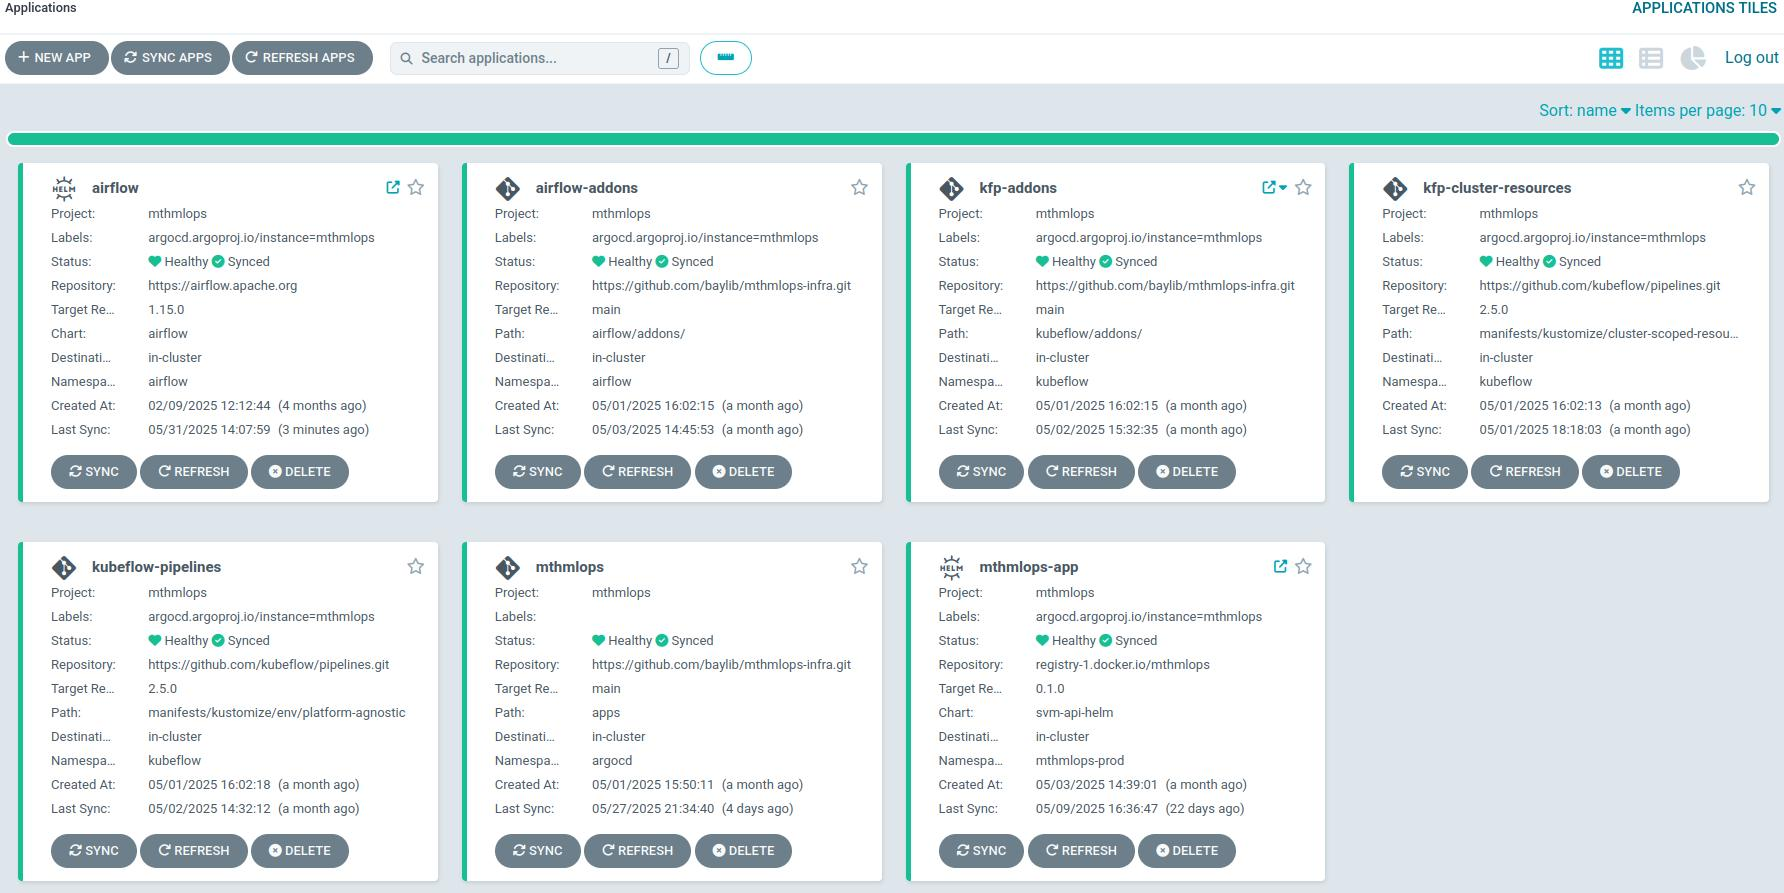
\includegraphics[width=\textwidth]{images/project/argocd-deployments}
    \label{fig:argocd-infra}
\end{figure}

Implementation details and usage instructions can be found in the corresponding GitHub repositories (refer to the annexes for links).
To support this setup, we created a dedicated ArgoCD project, allowing us to separate this ML workflow from other ML development projects.
Figure~\ref{fig:app-of-apps-pattern} displays our parent application, illustrating the use of the ArgoCD app-of-apps pattern.

\begin{figure}[!htbp]
    \centering
    \caption{ArgoCD App-of-apps pattern usage}
    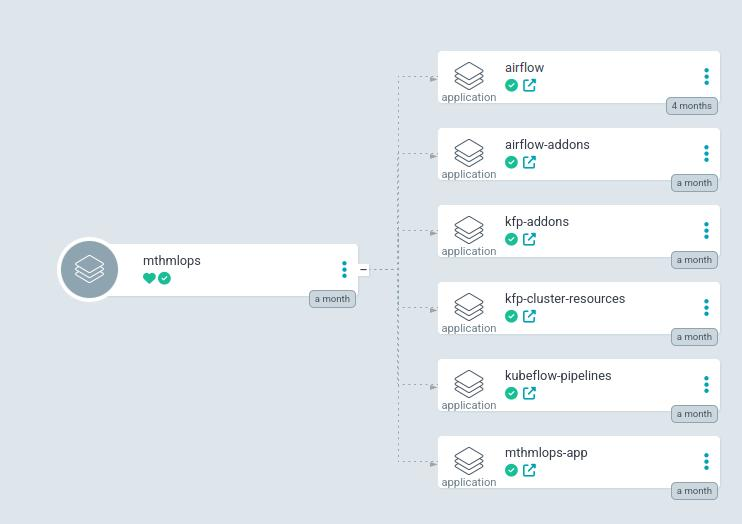
\includegraphics[scale=0.3]{images/project/app-of-apps-pattern}
    \label{fig:app-of-apps-pattern}
\end{figure}

\subsection{DataOps pipelines with Airflow}\label{subsec:dataops-pipelines2}
DataOps pipelines are defined as Airflow DAGs that leverage Airflow’s KubernetesExecutor, which creates a pod (i.e., a running container) for each step defined in the pipeline.

The goal is to deliver usable data into accessible storage for our Machine Learning Engineering teams.
In the initial iteration or development environment, this can be a local volume, with migration to external storage volumes planned later.
By using Kubernetes Persistent Volumes (PV) and Persistent Volume Claims (PVC), we can mount external S3-compatible storage in the same way.
Airflow’s Domain-Specific-Language also facilitates easier data storage management.

Steps in our DataOps pipeline can be integrated with an observability stack such as OpenSearch or Elasticsearch to analyze and store data.
These tools can also serve as monitoring solutions for our entire infrastructure.

\begin{figure}[!htbp]
    \centering
    \caption{Example of a pipeline define within Airflow}
    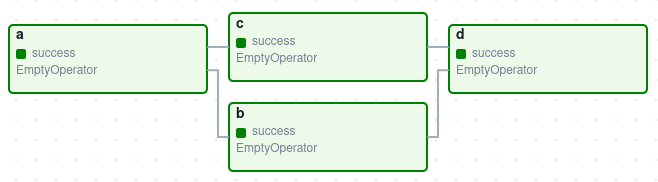
\includegraphics[scale=0.3]{images/project/data-ops-airflow-dag}
    \label{fig:project-data-ops-airflow-dag}
\end{figure}

\subsection{MLOps pipelines with Kubeflow}\label{subsec:mlops-pipelines2}
Within our infrastructure (see Figure~\ref{fig:project-infra}), Kubeflow enables us to deploy all the necessary steps of our MLOps pipeline by creating pods in the appropriate namespaces within our Kubernetes cluster—much like how Airflow manages our DataOps pipelines.
We use Kubeflow to provide our ML engineers with additional features such as model and metadata storage.
Furthermore, other components from the Kubeflow ecosystem can be integrated at any time if needed.

\begin{figure}[!htbp]
    \centering
    \caption{Example of a pipeline define within Kubeflow}
    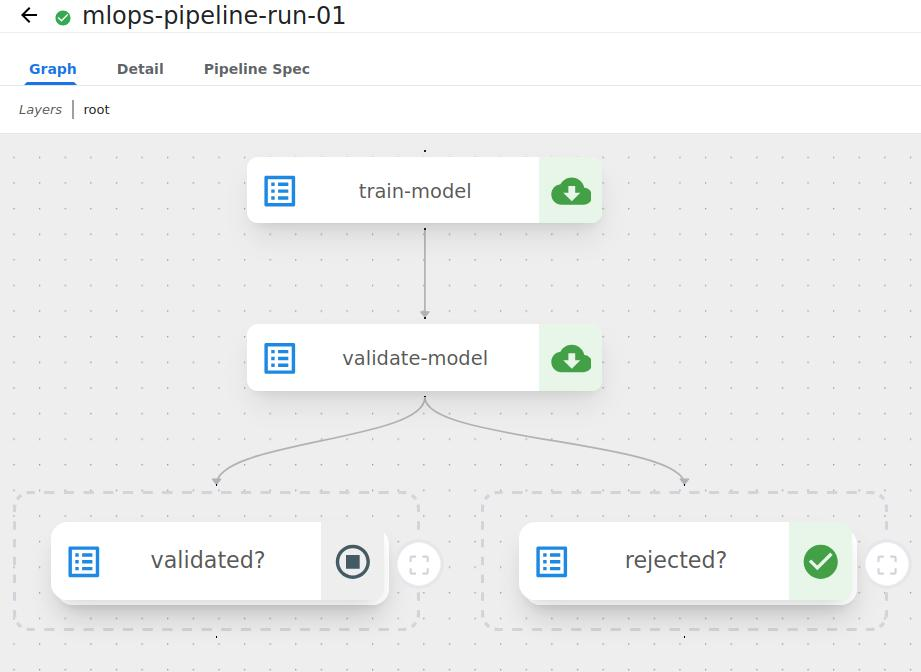
\includegraphics[scale=0.3]{images/project/mlops-workflow-kubeflow}
    \label{fig:project-ml-ops-airflow-dag}
\end{figure}

\subsection{Storages}\label{subsec:storage}
Here we describe the storage components in our infrastructure (Figure~\ref{fig:project-infra}) and their roles within our workflow.

\begin{itemize}
    \item \textbf{Model repository:} Managed by Kubeflow, this S3-compatible storage holds trained, pretrained, and untrained models.
    It can be mounted as a volume in Kubernetes and attached to running containers.
    \item \textbf{Image repository:} Stores container images that our cluster pulls during deployment.
    \item \textbf{Helm Chart repository:} Maintains and versions our infrastructure-as-code templates as Helm packages.
    \item \textbf{Metadata database:} Managed by Kubeflow, it stores model metadata and experiment tracking information.
    \item \textbf{Git repositories:} Store code and configuration, as described earlier.
    \item \textbf{Local volumes:} Used for storing other implementation-specific artifacts.
\end{itemize}

\subsection{Model development}\label{subsec:model-development}
As previously mentioned, we use Helm and Docker to package our model code.
In this section, we'll go into detail about how the model is defined.
The model's Docker image supports three operational modes, each configurable via parameters:
\begin{itemize}
    \item Training mode that loads and trains the untrained model on training data.
    \item A validation mode to load, test and validate the model.
    \item A listen mode define as a REST API server to interface with external frontends or services.
\end{itemize}

To integrate smoothly with our DataOps and MLOps pipelines, we define parameters that specify storage locations.
This ensures that any container image meeting these requirements can be seamlessly used within the pipeline.
Since we use the container layered model, it allows us to take any base image and add a layer that satisfies our pipeline's interface requirements.
While it's convenient to define all stages (training, validation, and listening) within a single image, it may be preferable to split them into two or three separate images.
One downside of the single-image approach is that the model's code is packaged into the same container that's deployed to production.

To deploy our production REST API server to Kubernetes, we created a standard Helm project with template manifests for a Service,
ServiceAccount, Ingress, and Deployment.
In the Helm (values.yaml) configuration file, we specify which trained model version should be loaded, allowing for seamless model hot-swapping when needed.
For more advanced deployment strategies, we can replace the standard Deployment manifest with a Rollout manifest (Custom Resource Definition (CRD) managed by Argo Rollouts).

To use the model within our MLops Kubeflow pipeline, we use our training and validation mode and our data location parameters with Kubeflow Domain specific language container components.
We use the same approach for our DataOps pipelines steps to ensure consistency as we'll demonstrate later in this paper.

Figure~\ref{fig:model-api} shows the model HelmChart and it's component deployed using ArgoCD\@.

% image of argocd api deployment.
\begin{figure}[!htbp]
    \centering
    \caption{Our model REST API HelmChart deployed using ArgoCD}
    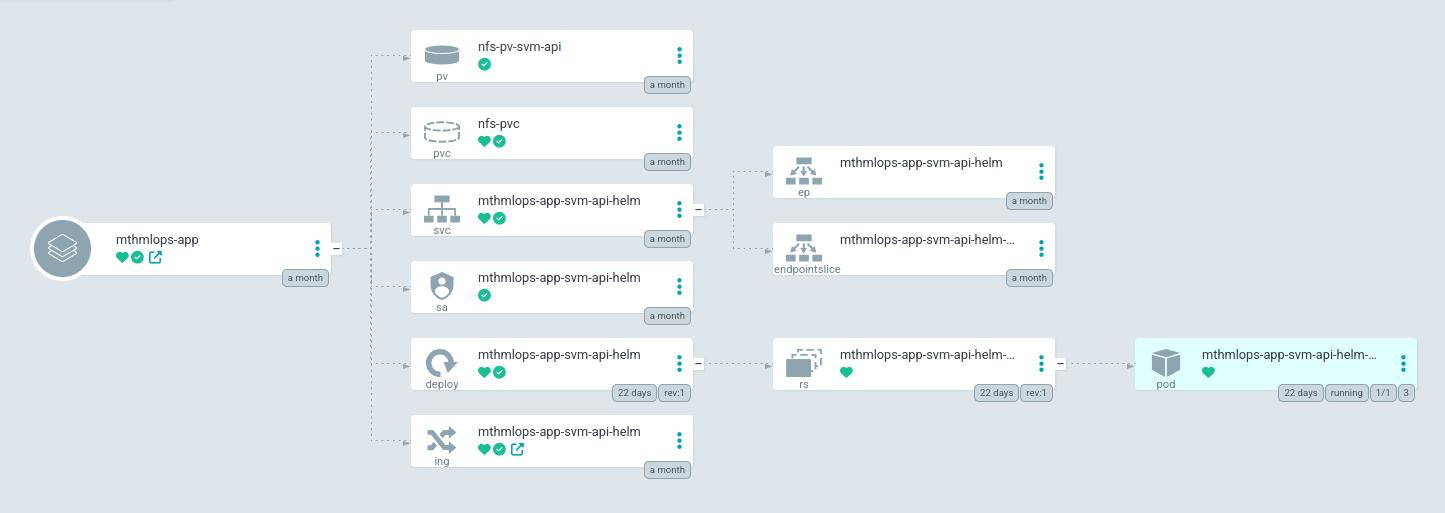
\includegraphics[width=\textwidth]{images/project/argocd-model-api}
    \label{fig:model-api}
\end{figure}
